\chapter{TINJAUAN PUSTAKA}

\section{Hasil Penelitian Terdahulu}
Terdapat penelitian terdahulu yang digunakan sebagai bahan studi literatur berdasarkan tema penelitian sejenis dan mendekati apa yang dibahas pada penelitian ini. Diantaranya dapat dilihat pada tabel \ref{table:Penelitian Terdahulu}.

\begin{longtable}{|c|m{0.2\linewidth}|m{0.6\linewidth}|}
  \caption{Penelitian terdahulu} \label{table:Penelitian Terdahulu} \\ \hline
  \multicolumn{1}{|c|}{\textbf{No}} & \multicolumn{1}{c|}{\textbf{Penulis dan Tahun Terbit}} & \multicolumn{1}{c|}{\textbf{Informasi Penelitian}} \\ \hline
  \endfirsthead
  \hline
  \multicolumn{1}{|c|}{\textbf{No}} & \multicolumn{1}{c|}{\textbf{Penulis dan Tahun Terbit}} & \multicolumn{1}{c|}{\textbf{Informasi Penelitian}} \\ \hline
  \endhead
  \hline
  \endfoot
  \hline
  \endlastfoot
  \multirow{2}{*}{1} & \multicolumn{2}{|p{\dimexpr0.9\linewidth}|}{\textit{The Artificial Bee Colony Algorithm: A Comprehensive Survey of Variants, Modifications, Applications, Developments, and Opportunities}} \\ \cline{2-3} 
                   & \multicolumn{1}{c|}{\parencite{Ibrahim2025}} & Penelitian ini menyajikan tinjauan komprehensif tentang algoritma \textit{Artificial Bee Colony} (ABC), termasuk variasi, modifikasi, aplikasi, dan perkembangan terkini dalam bidang optimasi. Fokus utama dari studi ini adalah untuk memberikan pemahaman yang lebih baik mengenai algoritma ABC, mengidentifikasi perbaikan yang telah dilakukan dalam algoritma ini, serta variasi dan adaptasi yang digunakan untuk meningkatkan kinerjanya. Studi ini juga mencakup tantangan yang dihadapi oleh ABC, termasuk konvergensi yang lambat dan kecenderungan untuk terjebak di solusi lokal, serta solusi yang diusulkan untuk mengatasi masalah tersebut, seperti peningkatan mekanisme pemilihan tetangga dan peningkatan fase eksploitasi. \\ \hline
  \pagebreak
  \multirow{2}{*}{2} & \multicolumn{2}{|p{\dimexpr0.9\linewidth}|}{\textit{Multi-objective Tasks Scheduling Using Bee Colony Algorithm in Cloud Computing}} \\ \cline{2-3}
                   & \multicolumn{1}{c|}{\parencite{Babadi2022}} & Penelitian ini memperkenalkan teknik baru untuk alokasi sumber daya pemrosesan yang tersedia berdasarkan algoritma \textit{Artificial Bee Colony} (ABC) untuk menyelesaikan masalah penjadwalan tugas di jaringan komputasi awan. Hasil penelitian menunjukkan kinerja metode yang diusulkan lebih baik dibandingkan dengan metode lainnya. Penelitian ini juga mengkaji penjadwalan tugas multi-objektif dengan menggunakan algoritma ABC yang terbukti efektif dalam mengalokasikan sumber daya pemrosesan secara efisien dalam lingkungan komputasi awan. Dalam beberapa studi terkait, fungsi \textit{fitness} yang digunakan untuk optimasi tugas multi-objektif melibatkan \textit{makespan} (waktu penyelesaian tugas) dan \textit{cost} (biaya operasional). Dengan pengujian yang dilakukan pada berbagai dataset, hasil menunjukkan bahwa metode ini menghasilkan waktu pemrosesan yang lebih cepat dan mengurangi konsumsi energi dibandingkan dengan metode alokasi acak, menjadikannya solusi yang lebih optimal untuk penjadwalan tugas di \textit{cloud computing}. \\ \hline
  \multirow{2}{*}{3} & \multicolumn{2}{|p{\dimexpr0.9\linewidth}|}{\textit{A Review on the Studies Employing Artificial Bee Colony Algorithm to Solve Combinatorial Optimization Problems}} \\ \cline{2-3}
                   & \multicolumn{1}{c|}{\parencite{Kaya2022}} & Studi ini mengulas 251 penelitian yang menggunakan algoritma \textit{Artificial Bee Colony} (ABC) untuk menyelesaikan masalah optimasi kombinatorial, seperti \textit{routing}, \textit{traveling salesman}, \textit{vehicle routing}, dan \textit{assembly/disassembly}. ABC yang banyak diterapkan dalam berbagai jenis masalah optimasi telah dimodifikasi dengan mekanisme tambahan untuk meningkatkan pencarian lokal. Pendekatan seleksi dan penentuan populasi awal bervariasi untuk meningkatkan kinerja algoritma. ABC adalah salah satu algoritma optimasi \textit{metaheuristik} berbasis \textit{Swarm Intelligence} yang populer dan telah digunakan untuk menyelesaikan banyak masalah dunia nyata. Studi ini menunjukkan keberhasilan ABC dalam berbagai jenis masalah dan potensi penelitian lebih lanjut pada area yang kurang dieksplorasi. \\ \hline
  \pagebreak
  \multirow{2}{*}{4} & \multicolumn{2}{|p{\dimexpr0.9\linewidth}|}{\textit{A Hyper-Parameter Optimizer Algorithm Based on Conditional Opposition Local-Based Learning Forbidden Redundant Indexes Adaptive Artificial Bee Colony Applied to Regularized Extreme Learning Machine}} \\ \cline{2-3}
                   & \multicolumn{1}{c|}{\parencite{Vasquez2024}} & Penelitian ini melakukan modifikasi algoritma \textit{Artificial Bee Colony} (ABC) untuk mengoptimalkan hiperparameter pada \textit{Regularized Extreme Learning Machine} (R-ELM). Modifikasi ini menggabungkan tiga metode, yaitu mekanisme adaptif untuk mengatur keseimbangan eksplorasi dan eksploitasi, \textit{Opposition Based-Learning} (OBL) untuk memperkuat eksploitasi, serta \textit{Forbidden Redundant Indexes} (FRI) untuk mencegah perhitungan berulang dan memaksimalkan efisiensi komputasi. Penelitian ini memberikan wawasan baru dalam pengoptimalan hiperparameter dalam waktu yang lebih efisien. \\ \hline
    \multirow{2}{*}{5} & \multicolumn{2}{|p{\dimexpr0.9\linewidth}|}{\textit{Exploring Swarm Intelligence Optimization Techniques for Task Scheduling in Cloud Computing Algorithms, Performance Analysis, and Future Prospects}} \\ \cline{2-3}
                   & \multicolumn{1}{c|}{\parencite{Prity2024}} & Penelitian ini memberikan tinjauan menyeluruh terhadap teknik optimisasi berbasis \textit{Swarm Intelligence} untuk penjadwalan tugas dalam komputasi awan. Studi ini menyebutkan penerapan algoritma seperti \textit{Particle Swarm Optimization} (PSO), \textit{Artificial Bee Colony} (ABC), dan \textit{Genetic Algorithm} (GA) dalam mengatasi tantangan penjadwalan tugas di lingkungan \textit{cloud}. Penelitian ini membahas bagaimana algoritma-algoritma tersebut dapat digunakan untuk mengoptimalkan alokasi sumber daya, meningkatkan kinerja sistem, dan memanfaatkan sumber daya secara efisien. Penelitian ini juga mengidentifikasi berbagai tantangan yang dihadapi dalam penerapannya, dan mengusulkan arah penelitian masa depan di bidang ini. \\ \hline
    \multirow{2}{*}{6} & \multicolumn{2}{|p{\dimexpr0.9\linewidth}|}{\textit{Metaheuristic Approaches in Path Finding and Optimization}} \\ \cline{2-3}
                   & \multicolumn{1}{c|}{\parencite{Trivedi2025}} & Penelitian ini membahas penerapan algoritma \textit{metaheuristik}. Algoritma yang dikaji dalam penelitian ini termasuk \textit{Artificial Bee Colony} (ABC), \textit{Particle Swarm Optimization} (PSO), dan \textit{Genetic Algorithm} (GA), yang merupakan contoh dari algoritma \textit{metaheuristik} yang terinspirasi oleh fenomena alam. Penelitian ini memberikan analisis mendalam tentang penerapan algoritma dalam pencarian jalur dan optimisasi. \\ \hline
    \pagebreak
    \multirow{2}{*}{7} & \multicolumn{2}{|p{\dimexpr0.9\linewidth}|}{\textit{An Enhanced Artificial Bee Colony Algorithm Based on Elimination History and Elite Correction}} \\ \cline{2-3}
                   & \multicolumn{1}{c|}{\parencite{Lei2024}} & Penelitian ini mengusulkan \textit{Artificial Bee Colony} (ABC) yang ditingkatkan berdasarkan \textit{elimination history} dan \textit{elite correction} (HeCABC) untuk mengatasi masalah konvergensi lambat dan akurasi rendah dalam optimasi masalah kompleks. HeCABC memperkenalkan dua persamaan pencarian yang berbeda, yaitu satu untuk eksplorasi yang menggunakan solusi inferior yang dihilangkan dan satu lagi untuk eksploitasi berbasis pada fusi informasi \textit{elite}. Selain itu, strategi \textit{elite correction} diterapkan untuk meningkatkan kualitas \textit{elite} dalam koloni dan menghindari konvergensi prematur. Penelitian ini juga menjelaskan bagaimana metode \textit{elite} individu digunakan untuk mengatur tingkat eksplorasi dan eksploitasi dalam koloni lebah, dengan cara menggabungkan informasi dari beberapa individu \textit{elite} untuk memperbaiki solusi yang lebih baik. \\ \hline
\end{longtable}

Penelitian-penelitian tersebut memberikan gambaran mengenai berbagai pendekatan dan metode yang telah diterapkan dalam penjadwalan tugas di lingkungan \textit{cloud}, serta memberikan dasar yang kuat untuk mengembangkan dan mengimplementasikan kombinasi algoritma \textit{Artificial Bee Colony} (ABC) dengan\textit{ Elite Opposition-Based Learning} (EOBL) dalam penelitian ini.

\section{Dasar Teori}
\subsection{\textit{Cloud Computing}}
\textit{Cloud computing} didefinisikan sebagai model penyediaan layanan komputasi yang memungkinkan pengguna untuk mengakses sumber daya secara praktis, di mana saja, dan kapan saja sesuai kebutuhan. Sumber daya ini mencakup jaringan, server, penyimpanan, hingga aplikasi, yang berada dalam sebuah \textit{shared pool}, dan dapat dikonfigurasi, disediakan, serta dilepaskan kembali dengan cepat tanpa memerlukan interaksi langsung dengan penyedia layanan atau manajemen yang rumit. Model ini didasarkan pada lima karakteristik utama, yaitu layanan mandiri sesuai permintaan yang memungkinkan pengguna mengelola sumber daya secara independen, akses jaringan yang luas dari berbagai perangkat, penggabungan sumber daya untuk melayani banyak pelanggan secara efisien, elastisitas cepat untuk penyesuaian kapasitas secara dinamis, serta layanan yang terukur untuk memantau dan mengontrol penggunaan \parencite{Marinescu2017}. \textit{Cloud computing} menawarkan beberapa model layanan seperti pada gambar \ref{figure:Cloud Computing Service Models}.

\newpage

\begin{figure} [H]
    \centering
    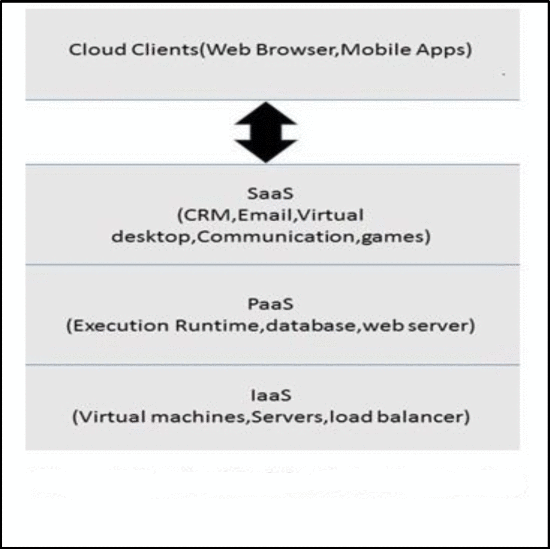
\includegraphics[width=0.75\linewidth]{gambar/Cloud Computing Service Models.png}
    \caption{\textit{Service models} pada \textit{cloud computing}}
    \label{figure:Cloud Computing Service Models}
\end{figure}

Model layanan pada \textit{cloud computing} menentukan tingkat kontrol pengguna atas sumber daya. Model pertama adalah \textit{Infrastructure as a Service} (IaaS), yang menyediakan entitas komputasi esensial seperti jaringan, penyimpanan, dan sumber daya komputasi lainnya. Pada model ini, pengguna tidak mengelola infrastruktur fisik \textit{cloud}, tetapi memiliki kontrol penuh atas sistem operasi, penyimpanan, dan aplikasi yang diimplementasikan, serta beberapa komponen jaringan tertentu. Model kedua, \textit{Platform as a Service} (PaaS), menyediakan platform berupa perangkat keras dan perangkat lunak yang dibutuhkan pengguna untuk mengembangkan dan menjalankan aplikasinya. Penyedia layanan mengelola infrastruktur secara keseluruhan, sehingga pengguna tidak perlu mengadakan perangkat keras atau perangkat lunak internal dan dapat fokus pada siklus pengembangan aplikasi. Model ketiga adalah \textit{Software as a Service} (SaaS), di mana pengguna dapat langsung mengakses dan menggunakan aplikasi perangkat lunak melalui internet dari berbagai perangkat. Layanan ini dikelola sepenuhnya oleh penyedia, termasuk pembaruan dan pemeliharaan, sehingga dapat diakses kapan saja dan dari mana saja \parencite{Sakshi2016}.

\subsection{\textit{Cloud Task Scheduling}}
\textit{Cloud task scheduling} adalah proses penentuan urutan dan alokasi tugas ke sumber daya komputasi yang tersedia dalam lingkungan \textit{cloud computing} untuk mencapai tujuan tertentu seperti minimalisasi \textit{makespan} (waktu penyelesaian total), peningkatan pemanfaatan sumber daya, dan pengurangan biaya operasi. Penjadwalan tugas merupakan salah satu aspek penting dalam \textit{cloud computing} untuk memastikan bahwa sumber daya komputasi digunakan secara efisien dan efektif \parencite{Awad2022}.

Konsep dasar \textit{cloud computing} menyediakan layanan komputasi melalui internet, yang mencakup infrastruktur, platform, dan aplikasi perangkat lunak. Dalam lingkungan \textit{cloud}, berbagai tugas dari banyak pengguna perlu dijadwalkan secara optimal pada sumber daya komputasi yang tersedia, baik itu mesin fisik maupun mesin virtual. Penjadwalan tugas di \textit{cloud} melibatkan pengelolaan tugas-tugas dari berbagai pengguna untuk menggunakan sumber daya secara efisien dalam lingkungan yang bersifat dinamis dan terdistribusi \parencite{Buyya2009}.

\subsection{\textit{Swarm Intelligence}}
\textit{Swarm Intelligence} adalah pendekatan kecerdasan buatan yang terinspirasi oleh perilaku kolektif dari sistem desentralisasi seperti kawanan burung, koloni semut, dan kawanan ikan. Prinsip dasar dari \textit{Swarm Intelligence} meliputi desentralisasi, interaksi lokal, dan emergensi, di mana perilaku global yang kompleks muncul dari interaksi sederhana antara agen individu. Algoritma yang terkenal dalam \textit{Swarm Intelligence} mencakup \textit{Ant Colony Optimization} (ACO), \textit{Particle Swarm Optimization} (PSO), dan \textit{Artificial Bee Colony} (ABC). Masing-masing algoritma ini meniru mekanisme alamiah untuk memecahkan masalah optimasi dengan cara yang adaptif.

Dalam konteks komputasi awan, \textit{Swarm Intelligence} telah diterapkan untuk penjadwalan tugas yang efisien dan penggunaan sumber daya yang optimal. Penelitian oleh Wang Xiang dan Wang Yancheng menunjukkan bahwa algoritma \textit{Swarm Intelligence}, seperti PSO dan ABC dapat secara signifikan meningkatkan efisiensi penjadwalan tugas di lingkungan \textit{cloud} dengan memperkenalkan strategi optimasi multi-objektif dan fungsi \textit{fitness} yang diperbaiki \parencite{Xiang2023}. Selain itu, algoritma ABC yang telah ditingkatkan menunjukkan kinerja yang lebih baik dalam hal mengurangi \textit{makespan} dan penyeimbangan beban pada mesin virtual di lingkungan \textit{cloud} yang heterogen \parencite{Kimpan2016}. \textit{Swarm Intelligence} menawarkan solusi yang adaptif dan efektif untuk berbagai tantangan kompleks dalam dunia komputasi awan.

\subsection{\textit{Artificial Bee Colony}}
\textit{Artificial Bee Colony} (ABC) adalah sebuah algoritma optimasi yang mekanismenya terinspirasi dari perilaku koloni lebah madu dalam mencari makan. Dalam analogi yang digunakan pada algoritma ini, posisi sumber makanan di alam direpresentasikan sebagai kandidat solusi dalam sebuah ruang pencarian. Koloni lebah di dalam algoritma ini terdiri dari tiga jenis lebah, yaitu \textit{employed bees} (lebah pekerja), \textit{onlooker bees} (lebah pengamat), dan \textit{scout bees} (lebah pengintai) \parencite{Wang2021}.

Setiap fase dalam algoritma ABC, memiliki rumus khusus yang digunakan untuk memodifikasi posisi solusi berdasarkan interaksi antara koloni lebah. Fase pertama dalam algoritma ini adalah fase \textit{employed bees}, di mana lebah pekerja mencari solusi yang lebih baik di sekitar solusi yang sedang dieksplorasi. Pada persamaaan \ref{equation:Fase Employed Bees ABC} menghitung posisi solusi baru.

\begin{equation}
\label{equation:Fase Employed Bees ABC}
    v_{mi} = x_{mi} + \varphi_{mi} \cdot (x_{mi} - x_{ki})
\end{equation}

Di mana \(v_{mi}\) adalah posisi sumber makanan baru yang dihasilkan, \(x_{mi}\) adalah posisi sumber makanan yang sedang dieksplorasi, \(x_{ki}\) adalah sumber makanan tetangga yang dipilih secara acak, \(\varphi_{mi}\) adalah nilai acak yang berada dalam rentang \([-a, a]\), dan \(a\) adalah parameter yang mengontrol ruang pencarian. Setelah menghasilkan sumber makanan baru, nilai \textit{fitness} dari solusi \(v_{mi}\) dihitung dan seleksi dengan metode \textit{greedy} yang diterapkan antara solusi \(v_{mi}\) dan \(x_{mi}\) untuk memilih solusi terbaik \parencite{Karaboga2010}.

Pada fase \textit{onlooker bees}, koloni lebah terdiri dari dua kelompok, yaitu lebah pengamat dan lebah pengintai. Lebah pekerja berbagi informasi mengenai sumber makanan yang mereka temukan dengan lebah pengamat yang berada di dalam sarang. Berdasarkan informasi ini, lebah pengamat kemudian memilih sumber makanan dengan probabilitas yang dihitung berdasarkan nilai \textit{fitness} yang diberikan oleh lebah pekerja. Untuk keperluan ini, digunakan metode seleksi berbasis \textit{fitness}, seperti seleksi roda \textit{roulette}, di mana nilai \textit{fitness} sumber makanan menjadi faktor utama dalam pemilihan solusi. Probabilitas \(p_{mi}\) dengan mana sumber makanan \(x_m\) dipilih oleh lebah pengamat dapat dihitung dengan menggunakan persamaan \ref{equation:Fase Onlooker Bees ABC} \parencite{Karaboga2010}.

\begin{equation}
\label{equation:Fase Onlooker Bees ABC}
    p_m = \frac{\text{fit}_m(x_m)}{\sum_{m=1}^{SN} \text{fit}_m(x_m)}
\end{equation}

Di mana \(\text{fit}_m(x_m)\) adalah nilai \textit{fitness} dari sumber makanan \(x_m\) pada iterasi ke-\(m\), dan \(SN\) adalah ukuran populasi sumber makanan. Setelah sumber makanan \(x_m\) dipilih secara probabilistik oleh lebah pengamat, sebuah sumber makanan tetangga \(v_m\) ditentukan menggunakan persamaan \ref{equation:Fase Employed Bees ABC}, dan nilai \textit{fitness} nya dihitung.

Pada fase \textit{scout bees}, lebah yang tidak dapat meningkatkan solusi mereka melalui sejumlah percobaan yang telah ditentukan, yang disebut dengan \textit{limit}, akan bertransformasi menjadi lebah pengintai. Lebah pekerja yang solusinya tidak dapat diperbaiki dalam jumlah percobaan yang telah ditetapkan oleh pengguna algoritma ABC, akan dianggap sebagai lebah pengintai, dan solusi yang mereka bawa akan ditinggalkan. Setelah itu, lebah pengintai mulai mencari solusi baru secara acak. Misalnya, jika solusi \( x_m \) telah ditinggalkan, solusi baru yang ditemukan oleh lebah pengintai yang sebelumnya merupakan lebah pekerja dari \( x_m \) akan menggantikan solusi yang telah ditinggalkan tersebut. Proses ini memastikan bahwa solusi yang awalnya buruk atau telah menjadi buruk akibat eksploitasi, akan digantikan dengan solusi baru yang lebih baik, menghindari terjebaknya algoritma dalam solusi yang tidak optimal \parencite{Karaboga2010}. 

ABC telah diterapkan dalam berbagai masalah optimasi, termasuk penjadwalan tugas di \textit{cloud}. Algoritma ini menunjukkan kemampuan untuk menemukan solusi global dan menghindari perangkap lokal, yang menjadikannya cocok untuk lingkungan komputasi yang dinamis dan kompleks. Penelitian yang dilakukan oleh Warangkhana Kimpan dan Boonhatai Kruekaew menunjukkan bahwa algoritma ABC dapat digunakan untuk penjadwalan tugas pada mesin virtual di \textit{cloud computing}. Mereka memperkenalkan \textit{heuristic task scheduling} dengan algoritma ABC untuk mesin virtual dalam lingkungan \textit{cloud} yang heterogen. Hasil eksperimen menunjukkan bahwa penggunaan ABC dapat meningkatkan efisiensi penjadwalan tugas dan penyeimbangan beban mesin virtual, serta meminimalkan \textit{makespan} \parencite{Kimpan2016}.

\subsection{\textit{Particle Swarm Optimization} (PSO)}
\textit{Particle Swarm Optimization} (PSO) merupakan algoritma optimasi yang dirancang untuk menyelesaikan masalah optimasi kontinu. Berbeda dengan algoritma genetika (\textit{Genetic Algorithm}) yang terinspirasi dari teori evolusi Darwin, PSO mengambil inspirasi dari perilaku sosial kawanan burung dalam mencari lokasi pendaratan terbaik. Dalam konteks ini, gerakan partikel dalam PSO diibaratkan sebagai kawanan burung yang secara sinkron bergerak untuk menentukan tempat pendaratan yang optimal dengan mempertimbangkan berbagai faktor, seperti ketersediaan makanan atau risiko predator. Karena terinspirasi oleh perilaku sosial, PSO diklasifikasikan sebagai bagian dari algoritma \textit{Swarm Intelligence} \parencite{Vanneschi2023}.

\subsection{\textit{Genetic Algorihm} (GA)}
\textit{Genetic Algorithm} (GA) merupakan keluarga model komputasi yang terinspirasi oleh proses evolusi biologis. Algoritma ini merepresentasikan solusi potensial untuk suatu masalah dalam bentuk struktur data yang menyerupai kromosom sederhana. GA menggunakan operator rekombinasi untuk memanipulasi struktur ini dengan tujuan mempertahankan informasi penting yang dapat meningkatkan kualitas solusi. Proses GA dimulai dengan inisialisasi populasi yang terdiri dari kromosom-kromosom yang biasanya dipilih secara acak. Setiap kromosom dievaluasi untuk menentukan tingkat kecocokan \textit{fitness} terhadap masalah yang dihadapi. Berdasarkan evaluasi tersebut, kromosom yang mewakili solusi yang lebih baik mendapatkan peluang reproduksi yang lebih besar dibandingkan dengan kromosom yang kualitasnya lebih rendah. Dengan cara ini, GA secara bertahap mengarahkan populasi menuju solusi yang lebih optimal melalui mekanisme seleksi alam dan rekombinasi \parencite{Mathew2019}.

\subsection{CloudSim}
CloudSim adalah \textit{toolkit} simulasi yang dirancang untuk memodelkan dan mensimulasikan lingkungan komputasi awan. Dikembangkan oleh Buyya, CloudSim menyediakan platform bagi peneliti untuk menguji dan mengevaluasi berbagai algoritma penjadwalan sumber daya dan teknik manajemen tanpa memerlukan infrastruktur \textit{cloud} fisik. Ini memungkinkan eksperimen dilakukan dalam lingkungan yang terkendali dan hasilnya dapat direplikasi dengan mudah. CloudSim terdiri dari beberapa komponen utama seperti \textit{data center}, \textit{host}, \textit{virtual machine} (VM), \textit{cloudlet}, dan broker, yang semuanya bekerja sama untuk memodelkan infrastruktur dan layanan \textit{cloud} secara efisien \parencite{Buyya2009}.

Salah satu keunggulan CloudSim adalah kemampuannya untuk mensimulasikan berbagai skenario komputasi awan, termasuk pengelolaan beban kerja yang dinamis dan heterogen. Selain itu, CloudSim mendukung perluasan dan modifikasi, memungkinkan peneliti untuk menambahkan fungsionalitas baru atau menyesuaikan perilaku komponen yang ada sesuai dengan kebutuhan spesifik mereka. Penelitian oleh Long dan Zhao memperluas CloudSim dengan menambahkan fungsi manajemen replikasi data dan pengelolaan \textit{striping file}, meningkatkan kemampuannya untuk simulasi penyimpanan data \textit{cloud} \parencite{Long2012}. Fitur-fitur baru ini memungkinkan pengguna CloudSim untuk mengintegrasikan strategi manajemen replikasi dan tata letak \textit{file} ke dalam penjadwalan tugas \textit{cloud}, yang berguna untuk meningkatkan kinerja sistem secara keseluruhan.

\subsection{Docker}
Docker adalah sebuah alat yang memungkinkan proses pembuatan artefak aplikasi yang dapat didistribusikan dengan mudah, penerapan aplikasi secara skala besar di berbagai lingkungan, serta memperlancar alur kerja dan responsifitas organisasi pengembangan perangkat lunak yang mengadopsi metodologi \textit{agile}. Dengan Docker, aplikasi dan seluruh dependensinya dikemas dalam sebuah \textit{container} yang portabel dan terisolasi, sehingga dapat dijalankan konsisten di berbagai platform perangkat keras dan sistem operasi \parencite{Matthias2015}.

Pemilihan Docker sebagai alat \textit{containerization} dalam studi ini didasarkan pada kesederhanaannya, portabilitas yang tinggi, dukungan komunitas yang kuat, serta pangsa pasar yang dominan di bidang \textit{containerization} \parencite{Novotny2023}.

\subsection{\textit{Elite Opposition-Based Learning}}
\textit{Elite Opposition-Based Learning} (EOBL) adalah teknik optimasi yang dikembangkan untuk meningkatkan kinerja algoritma optimasi dengan memanfaatkan konsep pembelajaran berbasis oposisi. Teknik ini berfokus pada penggunaan solusi oposisi dari individu \textit{elite} terpilih dalam populasi saat ini untuk mempercepat konvergensi algoritma menuju solusi optimal. Dalam EOBL, solusi oposisi dihitung untuk beberapa individu \textit{elite} pada probabilitas tertentu, dan populasi oposisi yang dihasilkan bersaing dengan populasi asli untuk memberikan lebih banyak peluang menemukan solusi global\parencite{Rahnamayan2008}.

Penggunaan \textit{Elite Opposition-Based Learning} (EOBL) dalam optimasi penjadwalan tugas di lingkungan \textit{cloud} dapat meningkatkan keberagaman solusi dengan memanfaatkan konsep \textit{generation jumping}, yaitu mengatur probabilitas terjadinya operasi oposisi sebagai pola mutasi untuk mendorong eksplorasi solusi yang lebih luas. EOBL mengutamakan penggunaan individu \textit{elite} dari populasi saat ini, menggantikan individu biasa pada OBL konvensional, sehingga solusi oposisi yang dihasilkan lebih mungkin berada di wilayah yang lebih baik dan mendekati solusi global optimal. Pendekatan ini memungkinkan algoritma untuk mempercepat konvergensi menuju solusi optimal, membantu menghindari jebakan pada solusi lokal, dan secara potensial meningkatkan efisiensi dalam penjadwalan tugas seperti pengurangan \textit{imbalance degree} \parencite{Zhou2013}.

\subsection{\textit{Dataset The san Diego Supercomputer} (SDSC) \textit{Blue Horizon Log}}
\textit{Dataset San Diego Supercomputer Center} (SDSC) \textit{Blue Horizon Log} merupakan kumpulan data rekaman jejak tugas (\textit{job trace}) yang dikumpulkan dari sistem Cray X-MP yang menjalankan sistem operasi CTSS pada bulan Oktober dan November 1989. Dataset ini mencakup lebih dari satu juta catatan tugas yang berisi informasi nama tugas, waktu mulai dan selesai, serta statistik pemakaian sumber daya seperti waktu CPU, waktu saluran input/\textit{output}, dan produk ruang-waktu memori. Untuk analisis, tugas-tugas diklasifikasikan berdasarkan nama perintah yang dijalankan, yang dibedakan menjadi perintah publik (dapat diakses oleh semua pengguna) dan perintah privat (khusus untuk pengguna tertentu). Karakterisasi statis dari dataset dilakukan dengan membuat representasi tugas rata-rata untuk setiap perintah, yang mewakili konsumsi sumber daya rata-rata dari seluruh tugas dengan nama perintah tersebut. Selanjutnya, tugas representatif ini diberi bobot sesuai dengan frekuensi relatif kemunculannya dalam keseluruhan data. Agar data lebih homogen dan \textit{outlier} dapat terisolasi, dilakukan transformasi logaritmik dan penskalaan. Data kemudian dikelompokkan menggunakan algoritma klaster \textit{k-means} dengan jarak \textit{euclidean} berbobot, mempertimbangkan tiga parameter utama pemakaian sumber daya, yaitu waktu CPU, waktu input/\textit{output}, dan produk ruang-waktu memori. Hasil klasterisasi ini membagi tugas menjadi tujuh klaster yang menggambarkan pola penggunaan sumber daya yang berbeda dalam sistem SDSC \textit{Blue Horizon} \parencite{Pasquale1988}.

\subsection{Parameter Penggunaan Sumber Daya \textit{Cloud}}
Beberapa parameter yang digunakan untuk menilai efisiensi dan kinerja sistem \textit{task scheduling} dalam pemanfaatan sumber daya \textit{cloud}.
\subsubsection{A. \textit{Makespan}}
\textit{Makespan} adalah interval waktu antara dimulainya tugas pertama hingga selesainya tugas terakhir dalam suatu proses penjadwalan. Nilai \textit{makespan} yang lebih kecil menunjukkan kinerja sistem yang lebih baik karena tugas dapat diselesaikan lebih cepat. Secara matematis, \textit{makespan} dinyatakan sebagai waktu penyelesaian maksimum dari seluruh tugas seperti pada persamaan \ref{equation:Makespan}.

\begin{equation}
\label{equation:Makespan}
    \text{\textit{Makespan}} = \max_{i \in \text{\textit{tasks}}} \{F_i\}
\end{equation}

Di mana $F_i$ adalah waktu penyelesaian (\textit{finishing time}) dari tugas ke-$i$ \parencite{Ciptaningtyas2024}.

\subsubsection{B. \textit{Average Start Time}}
\textit{Average start time} (waktu mulai rata-rata) adalah durasi rata-rata yang diperlukan untuk memulai pemrosesan semua tugas dalam sistem. Waktu mulai yang lebih awal menunjukkan efisiensi yang lebih baik dalam penjadwalan tugas. \textit{Average start time} dapat dihitung seperti pada persamaan \ref{equation:Average Start Time}.

\begin{equation}
\label{equation:Average Start Time}
    \text{\textit{Average start time}} = \frac{\sum_{i=1}^{n} \text{\textit{start time of} } R_i}{nR}
\end{equation}

Di mana $R_i$ adalah sumber daya ke-$i$, dan $nR$ adalah jumlah total sumber daya \parencite{Ciptaningtyas2024}.

\subsubsection{C. \textit{Average Finish Time}}
\textit{Average finish time} (waktu selesai rata-rata) adalah durasi rata-rata yang dibutuhkan untuk menyelesaikan seluruh tugas secara sukses. Waktu selesai yang lebih awal menunjukkan kinerja penjadwalan yang lebih baik. \textit{Average finish time} dapat dihitung seperti pada persamaan \ref{equation:Average Finish Time}.

\begin{equation}
\label{equation:Average Finish Time}
    \text{\textit{Average finish time}} = \frac{\sum_{i=1}^{n} \text{\textit{finish time of} } R_i}{nR}
\end{equation}

Di mana $R_i$ adalah sumber daya ke-$i$ dan $nR$ adalah jumlah total sumber daya \parencite{Ciptaningtyas2024}.

\subsubsection{D. \textit{Average Execution Time}}
\textit{Average execution time} (waktu eksekusi rata-rata) mengacu pada durasi rata-rata yang dibutuhkan untuk menyelesaikan suatu tugas tertentu. Waktu eksekusi yang lebih pendek menunjukkan efisiensi yang lebih baik dalam pelaksanaan tugas. \textit{Average execution time} dapat dihitung seperti pada persamaan \ref{equation:Average Execution Time}.

\begin{equation}
\label{equation:Average Execution Time}
    \text{\textit{Average execution time}} = \frac{\sum_{i=1}^{n} \text{times } T_i}{nT}
\end{equation}

Di mana $T_i$ adalah waktu penyelesaian tugas ke-$i$ dan $nT$ adalah jumlah total tugas \parencite{Ciptaningtyas2024}.

\subsubsection{E. \textit{Average Waiting Time}}
\textit{Average waiting time} adalah rata-rata waktu yang dibutuhkan oleh proses untuk menunggu sebelum dieksekusi dalam antrean. Waktu tunggu ini dihitung dari saat proses memasuki antrean hingga proses tersebut benar-benar dimulai. \textit{Average waiting time} memberikan gambaran seberapa efisien sistem dalam menangani antrean, di mana semakin kecil semakin cepat proses dapat dieksekusi setelah masuk antrean \parencite{Belferik2025}. Secara matematis, rumusnya seperti pada persamaan \ref{equation:Average Waiting Time}.

\begin{equation}
\label{equation:Average Waiting Time}
    \text {\textit{Average waiting time}} = \frac{\text{\textit{TotalDelay}}}{n}
\end{equation}

Untuk menghitung \textit{average waiting time}, kita menggunakan rumus yang lebih umum, yaitu dengan menjumlahkan seluruh \textit{waiting time} dari setiap proses dalam antrean, kemudian membaginya dengan jumlah total proses yang ada. 

\subsubsection{F. \textit{Scheduling Length}}
\textit{Scheduling length} merupakan jumlah total waktu penyelesaian seluruh tugas dalam sistem penjadwalan. Parameter ini mengukur keseluruhan durasi yang dihabiskan untuk mengeksekusi semua tugas, sehingga nilai yang lebih kecil menunjukkan efisiensi penjadwalan yang lebih baik. Secara matematis, \textit{scheduling length} ($SL$) dihitung sebagai total penjumlahan waktu penyelesaian semua tugas seperti pada persamaan \ref{equation:Scheduling Length} \parencite{Emara2021}.

\begin{equation}
\label{equation:Scheduling Length}
    \text{\textit{Scheduling length}} = \text {\textit{scheduling time}} + \textit{makespan}
\end{equation}

\subsubsection{G. \textit{Throughput}}
\textit{Throughput} adalah laju maksimum eksekusi tugas dalam satu satuan waktu. Dengan kata lain, \textit{throughput} mengukur jumlah total tugas yang berhasil diselesaikan per unit waktu. Parameter ini penting untuk menilai performa sistem dalam memproses tugas secara efisien. \textit{Throughput} dapat dihitung seperti pada persamaan \ref{equation:Throughput}.

\begin{equation}
\label{equation:Throughput}
    Throughput = \frac{nT}{makespan}
\end{equation}

Di mana $nT$ adalah jumlah total tugas yang diselesaikan dan $makespan$ adalah waktu penyelesaian tugas terakhir. Dengan nilai \textit{throughput} yang lebih tinggi, sistem dianggap mampu menyelesaikan lebih banyak tugas dalam waktu yang lebih singkat \parencite{Emara2021}.

\subsubsection{H. \textit{Resource Utilization}}
\textit{Resource utilization} (pemanfaatan sumber daya) mengukur efektivitas penggunaan sumber daya fisik, seperti CPU dalam sistem komputasi awan. Pemanfaatan CPU pada sumber daya fisik tertentu dihitung dengan menjumlahkan beban kerja dari setiap \textit{virtual machine}(VM) yang ditempatkan di sumber daya tersebut, lalu dibagi dengan kapasitas CPU sumber daya fisik tersebut. Dalam hal ini, VM yang ditempatkan di sumber daya tersebut dianggap memberikan kontribusi pada beban kerja total \parencite{Emara2021}. \textit{Resource utilization} secara matematis dapat dihitung seperti pada persamaan \ref{equation:Resource Utilization}.

\begin{equation}
\label{equation:Resource Utilization}
    \text{\textit{Resource utilization}} = \frac{\sum_{i=1}^{n} \text{\textit{finish time of} } R_i}{\text{\textit{makespan}} \times nR}
\end{equation}

\subsubsection{I. \textit{Energy Consumption}}
\textit{Energy consumption} (konsumsi energi) dalam sistem \textit{cloud computing} mengacu pada jumlah energi yang digunakan oleh sumber daya fisik untuk menjalankan tugas-tugas yang dialokasikan \parencite{Emara2021}.

\subsubsection{J. \textit{Imbalance Degree}}
\textit{Imbalance degree} (derajat ketidakseimbangan) mengukur seberapa merata distribusi beban kerja di antara \textit{virtual machine} (VM) dalam sistem \textit{cloud computing}, berdasarkan kemampuan eksekusi masing-masing VM. Untuk kebijakan penjadwalan yang ideal, nilai \textit{imbalance degree} harus serendah mungkin, karena nilai yang tinggi menunjukkan distribusi beban yang tidak merata yang dapat menyebabkan beban berlebih pada beberapa VM dan beban kurang pada VM lainnya \parencite{Tomar2022}. \textit{Imbalance degree} dapat dihitung seperti pada persamaan \ref{equation:Imbalance Degree}.

\begin{equation}
\label{equation:Imbalance Degree}
    \text{\textit{Imbalance degree}} = \frac{ET_{\max} - ET_{\min}}{ET_{\text{avg}}}
\end{equation}

di mana $ET_{\max}$ adalah waktu maksimum yang dihabiskan oleh VM dalam mengeksekusi semua \textit{cloudlet} yang diberikan, $ET_{\min}$ adalah waktu minimum, dan $ET_{\text{avg}}$ adalah waktu rata-rata eksekusi pada seluruh VM.